\section{Theory}

\textbf{(i)} The shallow water equations describe the flow of a thin layer of fluid under the influence of gravity and rotation. They consist of the momentum equations and the continuity equation and can be written as 
\begin{subequations}
\begin{empheq}[left=\empheqlbrace]{align}
    \frac{\partial u}{\partial t}& - fv = -g \frac{\partial \eta}{\partial x} \\
    \frac{\partial v}{\partial t}& + fu = -g \frac{\partial \eta}{\partial y} \\
    \frac{\partial \eta}{\partial t}& + H\left(\frac{\partial u}{\partial x} + \frac{\partial v}{\partial y}\right) = 0
\end{empheq}
\label{eq:SWE}
\end{subequations}
where $u$ and $v$ are the horizontal velocity components in the $x$ and $y$ directions. $\eta$ is the free surface height, $H$ is the mean fluid depth, $f=f_0$ is the constant Coriolis parameter on the f-plane, and $g$ is the acceleration due to gravity. The initial condition for the geostrophic adjustment problem can be seen in Figure \ref{fig:sketch}. The fluid is initially at rest $u(x,y,t=0)=v(x,y,t=0)=0$, and the free surface height has a step shape $\eta(x,y,t=0)=-\eta_0\text{sgn}(x)$. One can note that the intial condition is symmetric in $y$, and thus the solution will be independent of $y$. This allows us to reduce the problem by one dimension, i.e. $\tfrac{\partial}{\partial y}=0$. 
\begin{figure}[H]
    \centering    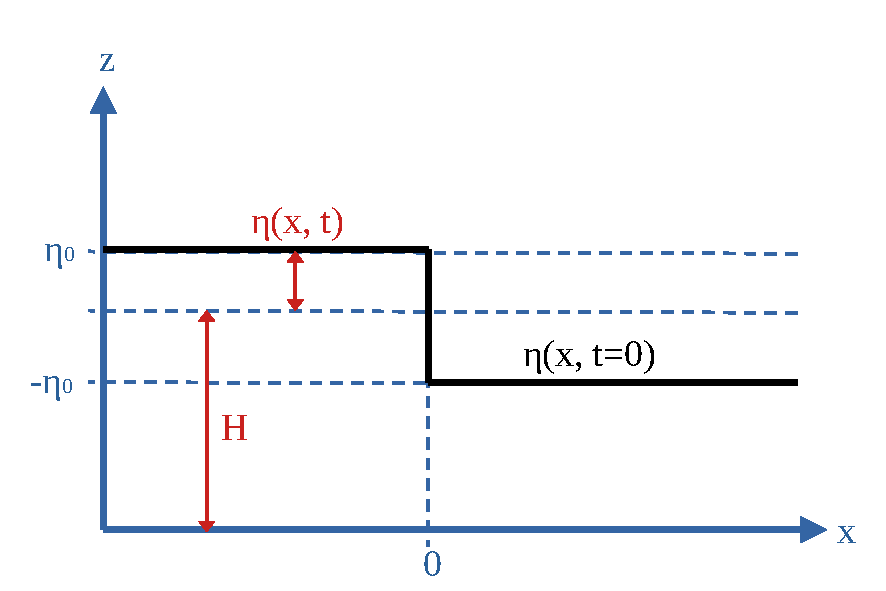
\includegraphics[width=0.6\textwidth]{Figures/sketch.pdf}
    \caption{This sketch shows the initial condition of the geostrophic adjustment problem. The fluid is initially at rest, and the free surface height has a step shape.}
    \label{fig:sketch}
\end{figure}

\textbf{(ii)} So the initial perturbation is a physical unstable state, which will start to move. The movement will start as a zonal, but it will start to turn due to the presence of the Coriolis force. Thus, a meridional wind will start to grow. This meridional wind can balance a certain amount of zonal height difference. Thus after a while the system will reach a steady state where the meridional flow will balance the remaining of the zonal height difference. The rest of the energy that moved away zonally will be 'lost energy', for the local system. 

The change in potential energy of the system is given by
\begin{equation}
    \begin{aligned}
    \Delta EP &= EP(t\rightarrow\infty)-EP(t=0)  =\frac{1}{2} g\rho \int_{-\infty}^{\infty}\int_{-\infty}^{\infty} \left[\eta(x,t\rightarrow\infty)^2-\eta(x,t=0)^2\right] dx\, dy \\ 
    &= -\frac{3}{2}g
    \rho g \eta_0^2 R L_y
    \end{aligned}
\end{equation}
The change in kinetic energy is given by
\begin{equation}
    \begin{aligned}
    \Delta EK &= EK(t\rightarrow\infty)-EK(t=0) = \frac{1}{2} \rho \int_{-\infty}^{\infty}\int_{-\infty}^{\infty} \left[v(x,t\rightarrow\infty)^2-0\right] dx \, dy \\
    &= \frac{1}{2} g\rho g \eta_0^2 R L_y
    \end{aligned}
\end{equation}
Thus the ratio of kinetic energy to potential energy is
\begin{equation}
    \frac{\Delta EK}{\Delta EP} = -\frac{1}{3}.
\end{equation}
One can furthermore express the final energy change as
\begin{equation}
    \Delta E = \Delta EP + \Delta EK = -\rho g \eta_0^2 R L_y.
\end{equation}
Since the initial state is no kinetic energy, one can see that a third of $\Delta EP$ is converted into $\Delta EK$, and the rest is lost. 

However above one must note a numerical models does not contain a infinite domain. Thus the above integrals should instead be evaluated over the finite domain of the numerical model, i.e. $\int_{-L_x/2}^{L_x/2}$. Using \autoref{eq:solh} one can integrate and get a proper solution on the finite domain. This gives
\begin{align}
    \Delta EP &= -\rho g\eta_0^2 L_y \left[-2Re^{-x/R}+\frac{R}{2}e^{-2x/R}\right]_0^{L_x/2} = -\rho g \eta_0^2 R L_y
\left(-2 e^{-L_x/(2R)} + \frac{1}{2} e^{-L_x/R} + \frac{3}{2}\right) \\ 
    \Delta EK &= HL_y\rho\left[\frac{g^2\eta_0^2}{f^2R^2}\left(-\frac{R}{2}e^{2x/R}\right)\right]_0^{L_x/2} = \frac{1}{2}g\rho g \eta_0^2 R L_y \left(1-e^{-\frac{L_x}{R}}\right). 
\end{align}
One can thus express a numerical energy change ratio as 
\begin{equation}
    \frac{\Delta EK}{\Delta EP} = -\frac{1}{3}\cdot\frac{1-e^{-\frac{L_x}{R}}}{-\tfrac{4}{3} e^{-L_x/(2R)} + \tfrac{1}{3} e^{-L_x/R} + 1}.
\end{equation}
On a finite domain one can also derive the total available potential energy in the initial state as 
\begin{equation}
    E_0 = \frac{1}{2}g\rho\eta_0^2L_xL_y.
\end{equation}

\textbf{(iii)} The final expression for the solution of the free surface height is given by
\begin{equation}
    \eta(x,t\rightarrow\infty) = \eta_0 \begin{cases}
        -1 + e^{-x/R} \quad \text{for } x \geq 0 \\
        1 - e^{x/R} \quad \text{for } x < 0.
    \end{cases}
    \label{eq:solh}
\end{equation}

Using this solution one can see that the zonal velocity is given $u(x,t\rightarrow\infty)=0$ and the meridional velocity is given by
\begin{equation}
    v(x,t\rightarrow\infty) = -\frac{g}{f}\frac{\partial \eta}{\partial x} = -\frac{g\eta_0}{f R} e^{-|x|/R}.
    \label{eq:solv}
\end{equation}
Note that the solutions are uniform in $y$, and will thus not depend on the variable. Above $g$ is the gravitational acceleration, $\eta_0$ is the initial height difference from the mean depth, $f$ is the Coriolis parameter, and $R$ is the Rossby radius of deformation. 

\textbf{(iv)} Observing \autoref{eq:solh} and \autoref{eq:solv} one can see that the solution is a function of the Rossby radius of deformation $R$. The Rossby radius of deformation is a length scale that characterizes the balance between the Coriolis force and the buoyancy due to the free surface height. The parameter $R$ is defined as $$R = \sqrt{gH}/f.$$ Since both \autoref{eq:solh} and \autoref{eq:solv} is proportional to $\propto e^{1/R}$, the Rossby radius will influence the extent of the solution. A larger Rossby radius will thus result in a larger distance needed to reach the boundary values of $\pm\eta_0$. Thus after a distance $x=R$ the solution will be 
\begin{equation}
    \eta(\pm R,t\rightarrow\infty) = \mp \eta_0 \left( 1 - \tfrac{1}{e} \right) \approx\mp 0.63 \eta_0.
\end{equation}
Thus increasing the depth by $4H$ or decreasing the Coriolis parameter by $\tfrac{1}{2}f$, would yield the same amount of broadening to the system. The gravity $g$ is also a parameter in the Rossby radius, but it is usually considered a constant. 

Finally the initial perturbation of $\eta_0$ will also affect the solution, as the limit when $x\rightarrow\pm\infty$ is approached. Consequently, this will equally scale the meridional velocity $v$ since $v\propto\eta_0$. However $v$ is also directly dependent as $v\propto\tfrac{1}{fR}$, which means that $v\propto\tfrac{1}{\sqrt{H}}$ but not dependent on $f$. Thus, varying the Coriolis parameter should vary the spread of the meridional velocity, but not the magnitude. Furthermore, varying the depth will also vary the spread, but also the the size of the magnitude $\abs{v}$.  